\subsection{\textit{Type Ia} : Combination of Buck and Boost Converter}

\subsection{\textit{Type Ia} : Combination of the Buck/Boost Converter :}
The figure\ref{fig:Type 1a Active Battery Balancing} illustrates the Type Ia balancing method for a battery system with n series-connected cells. The description is stack-to-cells-to-stack in accordance with the accepted nomenclature. A buck converter serves as a charging unit that distributes charge from the stack to the chosen cells. A boost converter reverses the process of discharge.
\\
The boost converter's input and output voltage ranges must be large enough to accommodate cells with voltages ranging from 1 to n-1. All cells can be actively charged and discharged up to the top level of the stack in this manner. It is only possible for nearby cells to balance numerous cells at once. Access to all cells below the topmost cell is used to balance that cell.
\\
This section explains the balancing procedure shown in Figure \ref{fig:Type 1a Active Battery Balancing}. The buck converter feeds Cell 1 with energy from the stack through switch \textit{$S_wA1$}. The converter output current $I_{Buck}$ is used to charge Cell 1. With the converter input current boost, the boost converter simultaneously discharges Cell 1 and Cell 2 through \textit{$S_wB2$}. The sum of the current in Cell 1 is 0A since $I_{Buck} = -I_{Boost} = I_{Bal}$, while Cell 2 discharges with $I_{boost}$A (negative balancing or "discharge mode"). The buck converter is often connected higher than the boost converter Batteries in Charging Mode. Discharging is done in the opposite order.
\\

\begin{figure}[h]
	\centering
	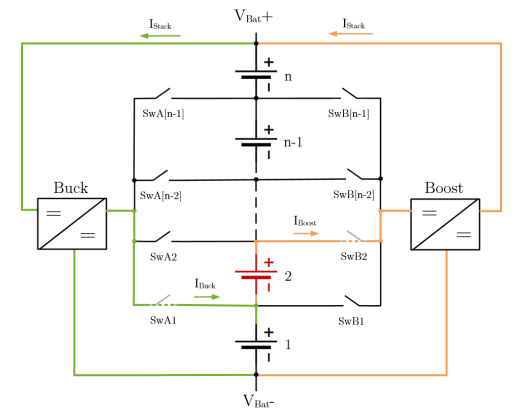
\includegraphics[width=0.7\textwidth]{Chap04/Figures/Type1a_ABMS.PNG}
	\caption{\textit{Type Ia}: Active Battery Balancing} 
	\label{fig:Type 1a Active Battery Balancing}
\end{figure}

The idle cell currents can be expressed as a vector following \ref{eq:Type1_cell_current}. It accounts for the balancing currents, both positive and negative, as well as the resulting stack current.
\begin{equation}\label{eq:Type1_cell_current}
    \vec{I_{Cell}}  = I_{stack} + \vec{I_n}\centerdot I_{Bal} - \vec{OUT}\centerdot I_{Bal}
\end{equation}

\begin{equation}\label{eq:Type1_cell_current}
    I_{stack}  = I_{Bal}(\frac{1}{\eta } \sum_{}^{}\vec{I_n}  - \eta\sum \vec{Out} ) \\
\end{equation}

\begin{equation}
\vec{OUT}  = \begin{pmatrix}
    S_{B1}\\
    \vdots
    S_{B[n-1]}  
\end{pmatrix} \\
, S_{x}=\left\{0\cdots1\right\}\\
, \vec{I_n}  = \begin{pmatrix}
    S_{A1}\\
    \vdots
    S_{A[n-1]}
\end{pmatrix} \\
\end{equation}

where $\vec{I_n}$ and $\vec{OUT}$ are the vectors of the switch signals $S_{A[x]}$ and $S_{B[x]}$ , respectively.
\\
The converter power and overall losses depend on the stack's n cells and the location of the balanced cell inside it. They rise as the position and the number of cells increases. \textit{I = J} when a single cell is in balance, In the absence of that, \textit{I} stands for the bottom cell of the balancing group and \textit{j} for the top one. As a result, \textit{I} and \textit{j} is always true.
\\
The necessary converters can be the traditional buck and boost converters depicted in Figures \ref{fig:Conventional Buck (a) and synchronous Buck(b) Conveter} and \ref{fig:Conventional Boost (a) and synchronous Boost(b) Conveter}. A synchronous design can be adopted, in which the diode is replaced with an actively regulated MOSFET to eliminate losses and to improve the efficiency of the converters across the whole operating range.
\begin{figure}[h]
	\centering
	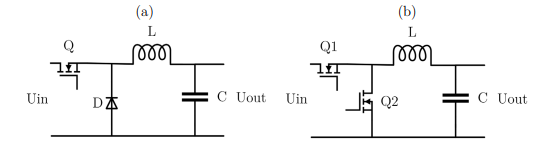
\includegraphics[width=0.9\textwidth]{Chap04/Figures/Conventiaonal_buck_synch_buck.PNG}
	\caption{Conventional Buck (a) and synchronous Buck(b) Conveter} 
	\label{fig:Conventional Buck (a) and synchronous Buck(b) Conveter}
\end{figure}

\begin{figure}[h]
	\centering
	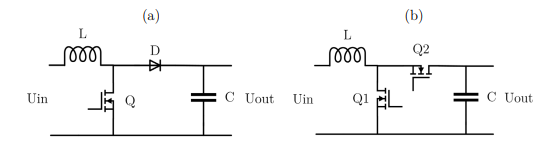
\includegraphics[width=0.9\textwidth]{Chap04/Figures/Conventiaonal_boost_synch_boost.PNG}
	\caption{Conventional Boost (a) and synchronous Boost(b) Conveter} 
	\label{fig:Conventional Boost (a) and synchronous Boost(b) Conveter}
\end{figure}

\subsection{\textit{Type Ib} : \textit{Type Ia} with a bidirectional converter :}
In terms of balancing routes, \textit{Type Ib} is comparable to \textit{Type Ia}. Bidirectional converters are used in place of unidirectional ones. Figure \ref{fig:Type1b Active Balancing Circuit } depicts the schematic for potential hardware implementation.\\

\subsection{\textit{Type IIa} :  Buck-boost converter :}
The Type IIa of the discussed balancing techniques is shown in Figure 50. Once more, n cells are arranged in series to make up the battery system. The description is cells-to-cells following the accepted nomenclature. This approach is comparable to cell bypassing if the load current and balancing current are the same. In discharge mode, a buck converter moves charge from one cell or many neighboring cells to its subjacent cells in the stack. A boost converter transfers charge in the other direction when it is in charge mode. A single bidirectional buck-boost converter can be created by combining the two converters.
\begin{figure}[h]
	\centering
	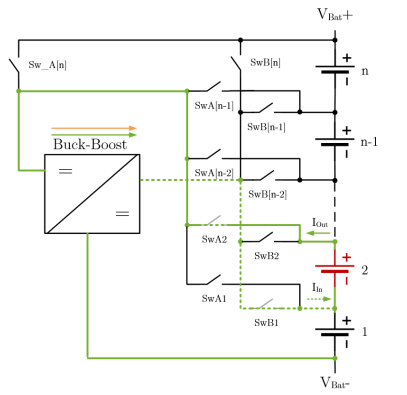
\includegraphics[width=0.6\textwidth]{Chap04/Figures/Type2a_ABMS.PNG}
	\caption{\textit{Type IIa} :  Buck-boost converter }
	\label{fig:Type2a Buck-boost converter}
\end{figure}
A bidirectional buck-boost converter made up of both converters is possible. To support 1 to n cells, the buck-boost converter's input and output voltage ranges must be sufficiently broad. Only cells that are close to one another can balance numerous cells at once. 
\\
\indent The explanation for the balancing procedure shown in Figure \ref{fig:Type2a Buck-boost converter} is given in the paragraphs that follow. Switches $S_{wA[2]}$ and $S_{wB[1]}$ in the buck converter allow the energy from Cells 1 and 2 to be transferred to Cell 1. 
it releases cells 1 and 2. The converter output current $I_{In}$ charges cell number one. In turn, Cell 1 is charged with $(I_{In} - I_{Out})$ A while Cell 2 is discharged with $I_{Out}$ A (negative balancing). $I_{Out}$ becomes $I_{Bal}$. 
In most cases, charging occurs when the DC/DC converter is connected in parallel to the desired cells and is in boost mode. However, in buck mode, discharge is performed in the same manner. Same charge and discharge operations as with \textit{Type I} are possible through switches $S_{wA[n]}$ and $S_{wB[n]}$.
\\
Depending on the number of balanced cells, the resulting cell current can be expressed as a vector:
\begin{equation}\label{eq:Type2_cell_current}
    \vec{I_{Cell}}  = \vec{I_{n}} \centerdot I_{Bal}  + \eta \centerdot \frac{\sum \vec{I_{n}}}{\sum \vec{I_{Out}}}\centerdot \vec{I_{Out}} \centerdot I_{Bal}
\end{equation}
\begin{equation}
    \vec{OUT}  = \begin{pmatrix}
        S_{B1}\\
        \vdots
        S_{Bn}  
    \end{pmatrix} \\
    , S_{x}=\left\{0\cdots1\right\}\\
    , \vec{I_n}  = \begin{pmatrix}
        S_{A1}\\
        \vdots
        S_{An}
    \end{pmatrix} \\
\end{equation}

\begin{figure}[h]
	\centering
	\subfigure[Conventional Buck-Boost Converter]{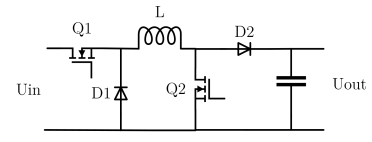
\includegraphics[scale=.7]{Chap04/Figures/Buck_boost_conventional.PNG}}
	\qquad
	\subfigure[Synchronous Buck-Boost Converter]{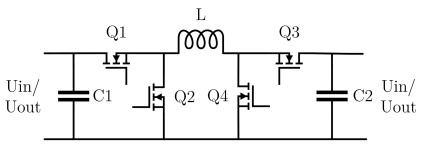
\includegraphics[scale=.7]{Chap04/Figures/Synchronous_buck_boost.PNG}}
	\caption{Typical Buck-Boost Converters}
	\label{fig:Type2a Typical Buck boost}
\end{figure}
Figure \ref{fig:Type2a Typical Buck boost}(a) depicts a potential buck-boost converter implementation. The N-MOSFET Q2 is disabled for buck mode, and Q1 is turned on and off. Q1 is constantly on in boost mode while Q2 is actively switched. The four-switch buck-boost converter from Figure \ref{fig:Type2a Typical Buck boost}(b)  may be used instead to enable synchronous mode.

\subsection{\textit{Type IIb} :  Bidirectional buck-boost converter :}
In terms of balancing routes, \textit{Type IIb} is comparable to \textit{Type IIa}. A bidirectional buck-boost converter is employed instead of a traditional (unidirectional) one. Because not every cell level requires a connection to both input and output, the number of MOSFETs needed in the switch-matrix is decreased. The same equations and exact operations are true for \textit{Type IIa} as well. Figure \ref{fig: Type2b active balancing architecture} displays the diagram and the power paths\cite{Active_Balancing_Thesis_Raber}[p. 60].
\begin{figure}[h]
	\centering
	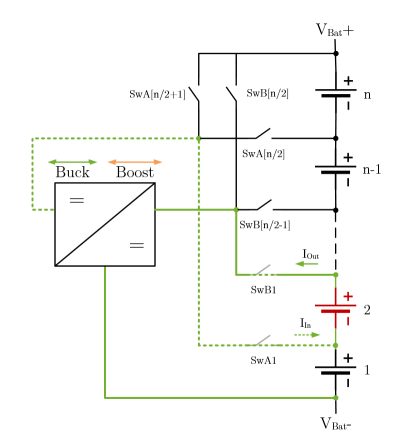
\includegraphics[width=.6\textwidth]{Chap04/Figures/Type2abABMS.PNG}
	\caption{\textit{Type IIb} active balancing architecture }
	\label{fig: Type2b active balancing architecture}
\end{figure}
A four-switch buck-boost converter similar to the one in Figure\ref{fig:Type2a Typical Buck boost}(b) can be used to realize the necessary bidirectional buck-boost converter. The ability to run the converter in a synchronous mode in both directions is a benefit of this design.


\subsection{\textit{Type IIIa} :  High - and low-side buck-boost converters :}
The system's implementation using high- and low-side buck-boost converters are shown in Figure \ref{fig:Type3a active balancing architecture}. Similar to \textit{Type I}, the operation involves the transfer of charge sequentially rather than simultaneously. There are two phases to the balancing process: one for the boost operation and one for the buck operation. The description is stack-to-cells-to-stack following accepted nomenclature. The high-side converter and low-side converter shouldn't work in the same direction at the same time to maintain a low average stack current throughout the two phases. To demonstrate how the high-side converter works in this example, balancing routes for \textit{Cell [n-1]} are also given in addition to \textit{Cell 2}\cite{Active_Balancing_Thesis_Raber}[p. 62].
Four converters, which can carry out the two phases concurrently, are used in an expanded version of this architecture\cite{Active_Balancing_Thesis_Raber}. There are more conceivable combinations: Another high-performance variant can be created by fusing the Type II concept with the Type III high-side converter.\\

\begin{figure}[h]
	\centering
	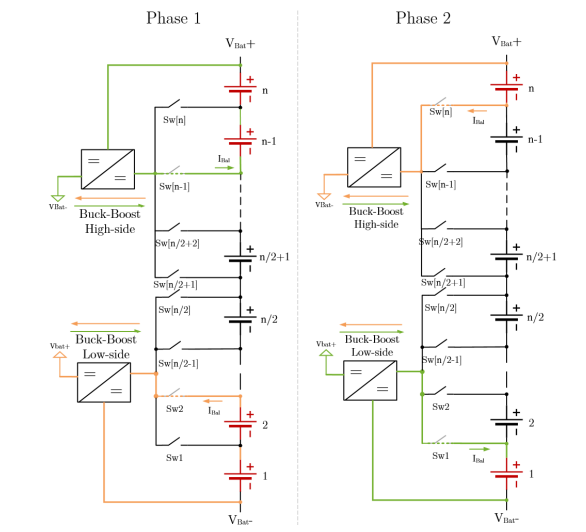
\includegraphics[width=0.6\textwidth]{Chap04/Figures/Type3a_ABMS.PNG}
	\caption{\textit{Type IIIa}  active balancing architecture}
	\label{fig:Type3a active balancing architecture}
\end{figure}
During Phase 1, the low-side converter functions as a boost converter, discharging \textit{Cells 1} and 2 through $S_{wA}$ with the converter's input current IBal, identical to Example \ref{fig:Type3a active balancing architecture}. \textit{Cell [n-1]} and \textit{Cell [n]} are simultaneously charged with IBal by the high-side converter while operating in buck mode. Phase 2 involves charging Cell 1 in buck mode and discharging \textit{Cell [n]} in boost mode to achieve the same balancing results as in Section (Results will be published in the upcoming chapters ). $I_{Bal}$ is used to charge and discharge \textit{Cell [n-1]} and \textit{Cell 2}.\\
A common ground connection allows the low-side converter to access all cells up to the middle of the battery stack, including \textit{Cell [n/2]}. It can be executed as depicted in Figure \ref{fig:Typical Schematics of the Low side and High Side buck boost Converter}. The design is made simpler by the fact that the two operating modes are only required in one direction. To enable synchronous operation for both modes, only two MOSFETs are required. If switch Q1 is not controlled, the MOSFET's intrinsic antiparallel diode enables normal operation albeit with lower efficiency.\\
The remaining cells are connected to the high-side converter through a shared $V_{Bat+}$ link. It is similar to the common ground converter in terms of design, but it has a distinct structure (see Figure \ref{fig:Type3a active balancing architecture}).